\section{Annotating regions}
\label{regionannot}

So far, all \lang programs have been fully annotated with regions information.
We now show how to infer these regions annotations based on
optionally-annotated programs.
First, we extend the region annotation to $\region{S}{E}$ where $S$ is
a set of variables. This annotation, defined below, is equivalent to nested
region annotations for each individual variable.

\begin{align*}
  \region{\Sone x\BORROW;S}{e} &= \region{\Sone x\BORROW}{\region{S}{e}}& \region{\emptyset}{e} &= e\\
\end{align*}

\Cref{fig:region-annotation} define a rewriting relation $\RannotT{e}{e'}$
which indicates that an optionally annotated term $e$ can be written
in a fully annotated term $e'$.
Through the rule \textsc{Rewrite-Top}, this is defined
in term of an inductively defined relation
$\Rannot{e}{e'}{S}$ where $n$ is the current nesting and $S$ is a set of
variable that are not enclosed in a region yet.
The base cases are constants, variables and borrows.
The general idea is to start from the leafs of the syntax tree, create a
region for each borrow, and enlarge the region as much as possible.
This is implemented by a depth-first walk of the syntax
tree which collects each variable that has a corresponding borrow.
At each step, it rewrites the inner subterms,
consider which borrow must be enclosed by a region now, and
return the others for later enclosing. Binders force immediate
enclosing of the bound variables, as demonstrated in rule \textsc{Rewrite-Lam}.
For nodes with multiple children, we
use a scope merge operator to decide if regions should be placed and where.
This is shown in rule \textsc{Rewrite-Pair}.
The merge operator, written $\getBorrows{B_l}{B_r}{(S_l,S,S_r)}$, takes
the sets $B_l$ and $B_r$ returned by rewriting the subterms
and returns three sets: $S_l$ and $S_r$ indicates the variables
that should be immediately enclosed by a region on the left and right
subterms and $S$ indicates the set of the yet-to-be-enclosed variables.
As an example, the rule \textsc{AnnotRegion-MutLeft} is applied
when there is an immutable borrow and a mutable borrow. In that case, a
region is created to enclose the immutable borrow, while the mutable
borrow is left to be closed later. This is coherent with the rules
for environment splitting and suspended bindings from \cref{sdtyping}.
%
Explicitly annotated regions are handled specially through
rule \textsc{Rewrite-Region}. In that case, we assume that all inner
borrows should be enclosed immediately.

\begin{figure*}[!hbt]
  \centering
  \begin{mathpar}
  \inferrule[AnnotRegion-Empty]{}{
    \getBorrows{\Sempty}{\Sempty}{\Sempty,\Sempty,\Sempty}
  }

  \inferrule[AnnotRegion-Nonempty]{
    \getBorrows{B_1}{B_2}{S_1,S,S_2}\\
    \getBorrows{b_1}{b_2}{S'_1,S',S'_2}
  }{
    \getBorrows{B_1;b_1}{B_2;b_2}
    {S_1\Sunion S'_1,S\Sunion S',S_2\Sunion S'_2}
  }
\end{mathpar}
\hrulefill
\begin{mathpar}
  \inferrule[AnnotRegion-Left]{}{
    \getBorrows
    {\Sone{x}{b}}
    {\Cempty}
    {\Cempty,\Sone{x}{b},\Cempty}
  }
  
  \inferrule[AnnotRegion-Right]{}{
    \getBorrows
    {\Cempty}
    {\Sone{x}{b}}
    {\Cempty,\Sone{x}{b},\Cempty}
  }
  
  \inferrule[AnnotRegion-Immut]{}{
    \getBorrows
    {\Sone{x}{\IBORROW}}
    {\Sone{x}{\IBORROW}}
    {\Cempty,\Sone{x}{\IBORROW},\Cempty}
  }
  
  \inferrule[AnnotRegion-MutLeft]{}{
    \getBorrows
    {\Sone{x}{\IBORROW}}
    {\Sone{x}{\MBORROW}}
    {\Sone{x}{\IBORROW},\Sone{x}{\MBORROW},\Cempty}
  }
  
  \inferrule[AnnotRegion-MutRight]{}{
    \getBorrows
    {\Sone{x}{\MBORROW}}
    {\Sone{x}{b}}
    {\Sone{x}{\MBORROW},\Cempty,\Sone{x}{b}}
  }
  
\end{mathpar}
\hrulefill
\begin{mathpar}
  \inferrule
  { e = \borrow{x} \mid \reborrow{x}}
  { \Rannot{e}{e}{\Sone{x}{b}} }

  \inferrule{e = c\ |\ x}
  { \Rannot{e}{e}{\Sempty} }

  \inferrule
  { \forall i,\ \Rannot{e_i}{e'_i}{B_i} \\
    \getBorrows{B_1}{B_2}{S_1,S,S_2}
  }
  { \Rannot{\app{e_1}{e_2}}{\app{\region{S_1}{e'_1}}{\region{S_2}{e'_2}}}{S} }

  \inferrule
  { \forall i,\ \Rannot{e_i}{e'_i}{B_i} \\
    \getBorrows{B_1}{(B_2\Sdel{x})}{S_1,S,S_2} \\
    S'_2 = S_2\Sunion B_2\Sonly{x}
  }
  { \Rannot
    {\letin{x}{e_1}{e_2}}
    {\letin{x}{\region{S_1}{e'_1}}{\region{S'_2}{e'_2}}}{S} }
  

  \inferrule
  { \forall i,\ \Rannot{e_i}{e'_i}{B_i} \\
    \getBorrows{B_1}{(B_2\Sdel{x,y})}{S_1,S,S_2} \\
    S'_2 = S_2\Sunion B_2\Sonly{x,y}
  }
  { \Rannot
    {\matchin{x,y}{e_1}{e_2}}
    {\matchin{x,y}{\region{S_1}{e'_1}}{\region{S'_2}{e'_2}}}{S} }

  \inferrule[Rewrite-Region]
  { \Rannot{e}{e'}{B} }
  { \Rannot{\regionS{e}}{\region{B}{e'}}{\Sempty} }

  \inferrule[Rewrite-Lam]
  { \Rannot{e}{e'}{B} \\
  }
  { \Rannot{\lam{x}{e}}{\lam{x}{\region{B}{e'}}}{\Sempty} }

  \inferrule[Rewrite-Pair]
  { \forall i,\ \Rannot{e_i}{e'_i}{B_i} \\
    \getBorrows{B_1}{B_2}{S_1,S,S_2}
  }
  { \Rannot
    {\introPair{e_1}{e_2}}
    {\introPair{\region{S_1}{e'_1}}{\region{S_2}{e'_2}}}
    {S} }

  \inferrule[Rewrite-Top]
  { \Rannot[1]{e}{e'}{S} }
  { \RannotT{e}{\region[1]{S}{e'}} }
\end{mathpar}

%%% Local Variables:
%%% mode: latex
%%% TeX-master: "main"
%%% End:

  \caption{Automatic region annotation --- $\RannotT{e}{e'}$}
  \label{fig:region-annotation}
\end{figure*}


\section{Constraints}
\label{appendix:constraints}

% \newcommand\A{\mathcal A}
% \newcommand\SC{\mathcal S}

Let us note $\A$ our constraint system. The full grammar of constraints is
given in \cref{grammar:constraint}.
$\A$ is defined as the smallest cylindric term constraint system that
satisfies the axiom shown in \cref{rules:entail}.
We follows the traditional HM(X) formulation
with conjunctions, projections and type inequalities.
The new element specific to our approach are kind inequalities.
Entailment is noted $\entail{C}{D}$, where $D$ is a consequence of the
constraints $C$.
We say that $C$ and $D$ are equivalent, noted $C \equivC D$,
when $\entail{C}{D}$ and $\entail{D}{C}$.
\TODO{Give the cylindric properties ?}

\begin{figure}[btp]
  \centering
  \begin{align*}
    C &::= \Cleq{\tau_1}{\tau_2}
        \mid \Cleq{k_1}{k_2}
        \mid C_1 \Cand C_2
        \mid \Cproj{\tvar}{C}
        \mid \Cproj{\kvar}{C}
  \end{align*}
  \caption{The constraint language}
  \label{grammar:constraint}
  % \begin{minipage}{0.65\linewidth}
  \begin{mathpar}
    \inferrule[Lat-UAL]{}{\kun \lk \kaff \lk \klin}
    \and
    \inferrule[Lat-Level]{\mul \lk \mul' \and n \lk n'}{\mul_n \lk_\Lat \mul'_{n'}}
  \end{mathpar}
\end{minipage}~
\begin{minipage}{0.2\linewidth}
  \centering
  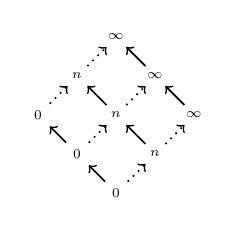
\begin{tikzpicture}
    [->,auto,semithick, every node/.style={scale=0.7}]
    \node(U) {$\kun_0$} ;
    \node(A) [above left of=U] {$\kaff_0$} ;
    \node(L) [above left of=A] {$\klin_0$} ;
    \node(Un) [above right of=U] {$\kun_n$} ;
    \node(An) [above left of=Un] {$\kaff_n$} ;
    \node(Ln) [above left of=An] {$\klin_n$} ;
    \node(Uinf) [above right of=Un] {$\kun_\infty$} ;
    \node(Ainf) [above left of=Uinf] {$\kaff_\infty$} ;
    \node(Linf) [above left of=Ainf] {$\klin_\infty$} ;
    \path
    (U) edge (A)
    (A) edge (L)
    (Un) edge (An)
    (An) edge (Ln)
    (Uinf) edge (Ainf)
    (Ainf) edge (Linf)
    ;
    \path[dotted]
    (U) edge (Un)
    (A) edge (An)
    (L) edge (Ln)
    (Un) edge (Uinf)
    (An) edge (Ainf)
    (Ln) edge (Linf)
    ;
  \end{tikzpicture}
\end{minipage}

%%% Local Variables:
%%% mode: latex
%%% TeX-master: "../main"
%%% End:

  % \caption{Lattice inequalities -- $k \lk_\Lat k'$}
  \begin{mathpar}
  \inferrule
  {}{ \entail{}{\Cleq{\kvar}{\kaff}} }
  \and
  \inferrule
  {}{ \entail{}{\Cleq{\kun}{\kvar}} }
  \and
  \inferrule
  {}{ \entail{}{\Cleq{\kvar}{\kvar}} }
  \and
  % \inferrule
  % {\Cleq{k}{k'} \in C}{ \entail{C}{\Cleq{k}{k'}} }
  % \and
  % \inferrule
  % { \entail{C}{\Cleq{x_1}{x}}\\
  %   \entail{C}{\Cleq{x}{x_2}}
  % }
  % { \entail{C}{\Cleq{x_1}{x_2}} }
  % \and
  % \inferrule
  % { \entail{C}{D} }
  % { \entail{C}{\Cproj{x}{D}} }
  % \\
  \inferrule
  { \entail{C}{\Cleq{\tau'_1}{\tau_1}}\\
    \entail{C}{\Cleq{\tau_2}{\tau'_2}}\\
    \entail{C}{\Cleq{k}{k'}}
  }
  { \entail{C}{\Cleq{\tau_1\tarr{k}\tau_2}{\tau'_1\tarr{k'}\tau'_2}} }
  \and
  \inferrule
  { \forall i,\ \entail{C}{\Cleq{\tau_i}{\tau_i}}\\
  }
  { \entail{C}{\Cleq{\tapp{t}{(\tau_i)}}{\tapp{t}{(\tau'_i)}}} }
  \and
  
  % \and
  % \inferrule
  % { \entail{C}{\Cleq{k}{k'}} \\
  %   \entail{C}{\Cleq{k'}{k}} }
  % { \entail{C}{\Ceq{k}{k'}} }
  % \and
  % \inferrule
  % { \entail{C}{\Cleq{k}{k'}} }
  % { \entail{C}{\Ckind{\tau_0\tarr{k}\tau_1}}{k'}}
  % \and
  % \text{Completion to form a cylindric constraint system.}
\end{mathpar}

%%% Local Variables:
%%% mode: latex
%%% TeX-master: "../main"
%%% End:

  \caption{Base entailment rules -- $\entail{C}{D}$ }
  \label{rules:entail}
\end{figure}


We note $\SC$ the set of solved forms
which can be used inside type and kind schemes.
We define $\SC$ as $\A$ quotiented by the relation $\equivC$.
%
The normalization function is described in \cref{infer:solving}.

% We consider the existence of a function $\operatorname{normalize}$ which takes
% a constraint in $\A$ and a substitution $\psi$ and returns a constraint
% in solved form $C' \in \SC$,
% and an updated substitution. We detail the implementation
% of the normalization function in \cref{infer:solving}

% $\mathcal S$ is composed only of kind
% inequalities \emph{over variables}. For convenience, if $C\in\mathcal S$, we
% note $C$ as a list of kind inequalities: $\Cleq{\kvar_i}{\kvar_{i'}}^n$.
% \TODO{Extend the properties of solved forms}

Our goal is to prove that $\CL$ supports all the properties necessary for
principal type inference, as defined by HM(X).

In order to prove this, we first prove that constraint solving
does compute normal forms, and that such normal forms are unique.


\begin{lemma}[Normal form]
  \label{lemma:normalform}
  Given a constraint $D\in\CL$, a substitution $\phi$ and
  $(C,\unif) = \normalize{D}{\phi}$,
  then $\phi\leq\unif$,
  $C \equivC \unif D$ and
  $\unif C = C$.
\end{lemma}
\begin{proof}
  % For simplicity, we assume that any substitution has been already applied
  % to $D$ and that $\phi = id$.
  Let us partition $\phi$ into a part which affects type variables,
  $\phi_\tau$, and a part which affects kind variables, $\phi_k$.
  
  We note $(C^k,\unif_\tau)$ the result of
  the modified Herbrand unification on $(D,\phi)$ in step (1).
  Herbrand unification computes the most general
  unifier. Our modified Herbrand unification only output additional
  kind constraints for kind on the arrows and does not change
  the result of the unification. Thus, we have
  $\phi_\tau\leq\unif_\tau$,
  $C^k \equivC \unif_\tau D$ and
  $\unif_\tau C^k = C^k$.
  
  Let $C^{k+}$ be the result after step (2), we trivially have that
  $\fv{C^{k+}} = \fv{C^k}$ and that $C^{k+} \equivC C^k$.

  Let $C^{A}$ and $\unif_k$ be the results after step (4).
  By definition, we have $\unif_k C^{k+} \equivC C^{A}$ and
  $\unif_k C^{A} = C^{A}$. Since $\phi_k$ has already be applied to $C$ before
  unifying the strongly connected components,
  we have that $\phi_k\leq\unif_k$.

  Let $\unif = \unif_\tau \meet \unif_k$. Since $\unif_\tau$ and $\unif_k$
  have disjoint supports,
  we have $C^{A} = \unif_\tau C^{A} \equivC \unif C^{k+} \equivC \unif D$
  and $\unif C^{A} = C^{A}$.
  Furthermore, $\phi_\tau \meet \phi_k \leq \unif_\tau \meet \unif_k$.
  
  Steps (5) to (9) all preserve the free variables and the equivalence
  of constraints, which concludes.
\end{proof}

\begin{lemma}[Uniqueness]
  Given $(C_1,\unif_1)$ and $(C_2,\unif_2)$ such that
  $\unif_1 C_1 \equivC \unif_2 C_2$, then
  $\normalize{C_1}{\unif_1}$ and $\normalize{C_2}{\unif_2}$
  are identical up to $\alpha$-renaming.
\end{lemma}
\begin{proof}
  In \cref{lemma:normalform}, we have showed that all the steps of the
  normalization procedure preserve equivalence.
  Since $\unif_1 C_1 \equivC \unif_2 C_2$, equivalence between
  the two results of the normalization procedures is preserved for all steps.

  We note $P(C_a)$ if for all $C = (k, k)'$
  such that $\entail{C_a}{C}$ and $\nvdash_eC$,
  we have $C \in {\mathcal R}_a$. 

  Let us note $C_1'$ and $C_2'$ the constraints after step (4). $P(C_1')$ and
  $P(C_2')$ hold. Indeed, since $C_1'$ and $C_2'$ are only composed
  of existential quantifications and kind inequalities, the only rules
  that applies are transitivity and lattice inequalities.
  After step (2) and (5), the associated relations are fully saturated for these
  two rules, hence all inequalities that can be deduced from $C_a'$ are already
  present in the relation.

  The property $P$ is preserved by step (6) since we only remove
  inequalities that involve existentially quantified variables. Such
  inequalities could not be picked in $P$.
  % In (6) we only remove
  % trivial lattice inequalities.

  Let us note $C''_a$ for $a\in\{1,2\}$ the constraints after step (5).
  Since there are no more existential variables,
  we have $C''_a=(k_i,k'_i)_i=\mathcal R''_a$.
  For any $C=(k,k')$ such that $\entail{}{C}$ and $\entail{C''_a}{C}$,
  then $C \in (\leq) \subset {\mathcal R}''_a$.
  Indeed, the only trivial inequalities in our system are equalities of the form
  $(\kvar, \kvar)$, which were removed in step (4) and the lattice inequalities.

  Let us consider $C = (k,k') \in \mathcal R''_1$.
  Since $C''_1\equivC C''_2$, we have $\entail{C''_2}{C}$.
  If $\nvdash_e{C}$, by $P(C''_2)$ we have that
  $C\in R''_2$.
  If $\entail{}{C}$, then $C\in (\leq) \subset R''_2$.
  We conclude that $R''_1 \subset R''_2$.
  By symmetry, $R''_1 = R''_2$ and $C''_1 = C''_2$.

  This equality is preserved by step (7) and (8)
  since the transitive reduction of a directed acyclic graph is unique,
  which concludes.
\end{proof}

We can now prove all the necessary high level properties.

\begin{lemma}
  For all $C\in\mathcal S$, $\entail{C}{x = x}$ implies
  $\entail{}{x = x}$.
\end{lemma}
\begin{proof}
  By definition of $\operatorname{normalize}$, We have $C = \Cleq{k}{k'}_i$
  such that the underlying relation has no cycles.
  Thus, we can not deduce neither kind nor type equalities from $C$.
\end{proof}

\begin{property}
  $\CL$ is regular, ie, for $x, x'$ two types or kinds,
  $\entail{}{\Ceq{x}{x'}}$ implies
  $\fv{x} = \fv{x'}$
\end{property}
\begin{proof}
  The only equalities possibles are between variables (via symmetry) or
  between constants.
\end{proof}

Finally, we can conclude with all the properties we need for
HM(X):

\begin{theorem}
  $\CL$ has the principal constraint property,
  $\operatorname{normalize}$ computes principal normal forms for $\CL$
  and $\CL$ is regular.
\end{theorem}


This is sufficient to show that $HM(\CL)$ is principal. However,
we do not use HM(X) directly but an extended version with kind inference,
linear and affine types, and borrow.


\section{Syntax directed typing}
\label{appendix:sdtyping}

\subsection{Kinding}

We note $\inferSK{C}{\E}{\tau}{k}$
when $\tau$ has kind $k$ in environment $\E$ under constraints $C$.
The rules are shown in \cref{rules:sd-kinding}.
Kinds and types follow a small calculus with variables ($\tvar$,\dots),
functions (type constructors $\T{t}$), application ($\tapp{t}{\Multi{\tau}}$)
and primitives such as types for arrows ($\tau\tarr{k}\tau'$) and
borrows ($\borrowty{k}{\tau}$).
Kind checking can thus be done in a fairly straightforward, syntax-directed
fashion by simply following
the syntax of the types. Kind arrows can only appear when looking
up the kind scheme of a type constructor $\T t$. Kind arrows are forbidden
in any other contexts.


\begin{figure}[ht]
  \centering
  \begin{mathpar}
  \inferrule[KVar]
  { \bvar{\tvar}{k} \in \E }
  { \inferSK{C}{\E}{\tvar}{k}
  }
  \and
  \inferrule[KPair]
  { \forall i \quad
    \inferSK{C}{\E}{\tau_i}{k_i} \quad
    \inferSS{C}{\E}{k_i}{k}
  }
  { \inferSK{C}{\E}{\tyPair{\tau_1}{\tau_2}}{k} }
  \and
  \inferrule[KApp]
  { \bvar{\T{\tcon}}{
      \forall \Multi[i]\kvar.\ \qual{D}{(\Multi[j]{k'}) \karr k'}}
    \in \E \\
    \unif = \subst{\Multi[i]\kvar}{\Multi[i]k}{} \\
    \entail C {\unif D} \\
    \forall j\quad
    \inferSK{C}{\E}{\tau_j}{k_j}\quad
    \inferSS{C}{\E}{k_j}{\unif{k'_j}}
  }
  { \inferSK{C}{\E}{\tapp{\tcon}{\Multi[j]{\tau}}}{\unif{k'}} }
  \and
  \inferrule[KBorrow]
  {}{ \inferSK{C}{\E}{\borrowty{k}{\tau}}{k}}
  \and
  \inferrule[KArr]
  {}
  { \inferSK{C}{\E}{\tau_1 \tarr{k} \tau_2}{k} }
\end{mathpar}


%%% Local Variables:
%%% mode: latex
%%% TeX-master: "../main"
%%% End:

  \caption{Syntax-directed kinding rule --
    $\inferSK{C}{\E}{\tau}{k}$}
  \label{rules:sd-kinding}
\end{figure}

\subsection{Environments}
\label{typ:extra:envs}

\begin{figure}[tp]
  \begin{mathpar}
  \inferrule[ESplit-Empty]{}{
    \bsplit{\Cempty}\Eempty\Eempty\Eempty
  }

  \inferrule[ESplit-Nonempty]{
    \bsplit{C_1}{\E}{\E_1}{\E_2} \\
    \bsplit{C_2}{b}{b_1}{b_2}
  }{
    \bsplit{C_1\Cand C_2}{\E;b}{\E_1;b_1}{\E_2;b_2}
  }

  \inferrule[ESplit-Check]{
    \bsplit{D}{\E}{\E_1}{\E_2} \\
    \entail{C}{D}
  }{
    \lsplit{C}{\E}{\E_1}{\E_2}
  }
\end{mathpar}
\hrulefill
\begin{mathpar}
  \inferrule[BSplit-Both]{}{
    \bsplit {\Cleq{\schm}{\kun_\infty}}
    {\bvar{x}{\schm}} {\bvar{x}{\schm}} {\bvar{x}{\schm}}
  }

  \inferrule[BSplit-Left]{}{
    \bsplit {\Cempty} {\bvar{x}{\schm}} {\bvar{x}{\schm}} {\bnone}
  }

  \inferrule[BSplit-Right]{}{
    \bsplit {\Cempty} {\bvar{x}{\schm}} {\bnone} {\bvar{x}{\schm}}
  }

  \inferrule[BSplit-Imm-Borrow]{}{
    \bsplit {\Cempty}
    {\bvar{\borrow[\IBORROW]{x}}{\schm}}
    {\bvar{\borrow[\IBORROW]{x}}{\schm}}{\bvar{\borrow[\IBORROW]{x}}{\schm}}
  }

  \inferrule[BSplit-To-Borrow]{}{
    \bsplit {\Cempty}{\bvar x \schm}{\svar x \schm^n}{\bvar x \schm}
  }

  \inferrule[BSplit-To-Imm]{}{
    \bsplit {\Cempty}
    {\bvar{\borrow x} \schm}{\svar[\IBORROW] x \schm^n}{\bvar{\borrow x} \schm}
  }
\end{mathpar}
%%% Local Variables:
%%% mode: latex
%%% TeX-master: "../main"
%%% End:

  \caption{Splitting --- environments $\lsplit
    C\E\E\E$; binders $\bsplit Cbbb$}
  \label{fig:sd-splitting}
\end{figure}

\begin{figure}[tp]
  \begin{mathpar}
  \inferrule[EBorrow]{
    \bregion{C_r}{}{\svar{x}{\tau}^n}{b}
  }{
    \bregion{C_r}{x}{\E;\svar{x}{\tau}^n}{\E; b}
  }

  \inferrule[EBorrow-Check]{
    \entail{C}{D}\\\\
    \bregion{D}{x}{\E;\svar{x}{\tau}^n}{\E; b}
  }{
    \lregion{C}{x}{\E;\svar{x}{\tau}^n}{\E; b}
  }
  
  \inferrule[EBorrow-Binder]{
    \BORROW\in\left\{\kun,\kaff\right\}\\
    C = (\BORROW_n\lk k) \wedge (k \lk \BORROW_\infty)
  }{
    \bregion{C}{}
    {\svar[\BORROW]{x}{\tau}^n}
    {\bvar{\borrow[\BORROW]{x}}{\borrowty[\BORROW] k{\tau}}}
  }
\end{mathpar}
%%% Local Variables:
%%% mode: latex
%%% TeX-master: "../main"
%%% End:

  \caption{Borrowing --- environments $\lregion
    C{x}\E\E$; binders $\bregion C{x}bb$}
  \label{fig:sd-borrowing}
\end{figure}


\begin{figure}[!htb]
  \begin{mathpar}

  \inferrule{}{ \Cleq{\Eempty}{k} \Crewrite  \Cempty}

  \inferrule{
    \Cleq\E k \Crewrite  C \\ \E \vdash \Cleq B k \Crewrite  D
  }{
    \Cleq{\E; B}{k} \Crewrite  C \Cand D
  }

  \inferrule{
    \E \vdash \Cleq \schm k \Crewrite  C
  }{ \E \vdash \Cleq{\bvar x \schm}{k} \Crewrite  C}

  \inferrule{ }{
    \E \vdash \Cleq{\svar x \schm^n} k \Crewrite  \Cfalse
  }

  % \inferrule{}{\Cleq{\IBORROW^n} k \Crewrite  \Cleq{\kun_n} k}

  % \inferrule{}{\Cleq{\MBORROW^n} k \Crewrite  \Cleq{\kaff_n} k}

    \inferrule{
      \inferK{C \Cand C_x} \E \tau {k'} \\
      D = C \Cand C_x \Cand \Cleq{k'}k
    }{
      \E \vdash
      \Cleq{(\forall \kvar_i \forall (\tvar_j:k_j).\ \qual{C_x}{\tau})}{k} \Crewrite  D
    }
  \end{mathpar}

  \caption{Rewriting constraints on environments and types}
  \label{rule:typing:desugar}
\end{figure}


\subsection{Typing}

\begin{figure*}[tp]
  \begin{mathpar}
  \inferrule{}{ \Cleq{\Eempty}{k} \Crewrite  \Cempty}

  \inferrule{
    \Cleq\E k \Crewrite  C \\ \E \vdash \Cleq B k \Crewrite  D
  }{
    \Cleq{\E; B}{k} \Crewrite  C \Cand D
  }
  \\
  \inferrule{
    \E \vdash \Cleq \schm k \Crewrite  C
  }{ \E \vdash \Cleq{\bvar x \schm}{k} \Crewrite  C}

  \inferrule{
    \E \vdash \Cleq \schm k \Crewrite  C \\
    \Cleq{\BORROW^n} k  \Crewrite  D
  }{
    \E \vdash \Cleq{\svar x \schm^n} k \Crewrite  C \Cand D
  }
  \\
  \inferrule{}{\Cleq{\IBORROW^n} k \Crewrite  \Cleq{\kun_n} k}

  \inferrule{}{\Cleq{\MBORROW^n} k \Crewrite  \Cleq{\kaff_n} k}
  \\
  \inferrule{
    \E; \Multi{\bvar{\alpha}{k}} \vdash \Cleq\tau k \Crewrite  D
  }{
    \E \vdash \Cleq{\forall\Multi\kvar\forall\Multi{\bvar{\alpha}{k}}.(\qual{C}{\tau})}
    k \Crewrite  C \Cand D
  }

  \inferrule{}
  { \E \vdash \Cleq{ \tau_2\tarr{k'}\tau_1 } k \Crewrite  \Cleq{k'}k }

  \inferrule{
    \E(\tvar) = \kschm
  }
  { \E \vdash \Cleq{ \tvar} k \Crewrite  \Cleq\kschm k }

  \inferrule{
  }{ \E \vdash \Cleq{\tapp{t}{\Multi\tau}} k \Crewrite  ???}

  \inferrule{}{
    \E \vdash \Cleq{\borrowty {k'} {\tau}} k \Crewrite  \Cleq{k'}k
  }
\end{mathpar}

%%% Local Variables:
%%% mode: latex
%%% TeX-master: "../main"
%%% End:

  \caption{Rewriting constraints on environments and types}
  \label{fig:contraints-environments-types}
\end{figure*}
\begin{figure*}[tp]
  \begin{mathpar}
  \inferrule[Scheme]{
    \inferSK{C \Cand C_x} \E \tau {k'} \\
    \entail C {\Cleq{k'}k}
  }{
    \entail C {(\forall \kvar_i \forall (\tvar_j:k_j).\
      \qual{C_x}{\tau}) \le  k}
  }
\end{mathpar}
\hrulefill
\begin{mathpar}
  \inferrule[Var]
  { \bvar{x}{
      \forall \kvar_i \forall (\tvar_j:k_j).\ \qual{C_x}{\tau}
    }
    \in \E \\
    \unif = [\kvar_i\mapsto k_i,\tvar_j \mapsto \tau_j] \\
    \entail C {\unif(C_x)} \\
    % \addlin{
    %   \inferSK{C}{\E}{\unif \tau}{k_\tau}
    % }
  }
  { \inferS{C}{\E}{x}{\unif\tau}
  }
  \and
  \ruleSDLam
  \and
  \ruleSDApp
  \and
  \inferrule[Let]
  { \inferS{C \Cand D}{\E_1}{e_1}{\tau_1} \\
    \schm = \forall\Multi\kvar\forall\bvar{\Multi\tvar}{\Multi{
        k}}. \qual{D}{\tau_1}\\
    \{\Multi\kvar, \Multi\tvar\} = \fv{D, \tau_1} \setminus \fv{C, \E}
  \\
  \entail{C}{\exists\Multi\kvar\Multi\tvar.D} \\
    \inferS{C}{\E;\bvar{x}{\sigma}}{e_2}{\tau_2} \\
    \addlin{\lsplit{C}{\E}{\E_1}{\E_2}}\\
  }
  { \inferS{C}
    {\E}{\letin{x}{e_1}{e_2}}{\tau_2} }
  \and
  \inferrule[Pair]
  { \inferS{C}{\E_1}{e_1}{\tau_1} \\
    \inferS{C}{\E_2}{e_2}{\tau_2} \\
    \addlin{\lsplit{C}{\E}{\E_1}{\E_2}}
  }
  { \inferS{C}{\E}{\introPair{e_1}{e_2}}{\tyPair{\tau_1}{\tau_2}} }
  \and
  \inferrule[MatchPair]
  { 
    \inferS{C}{\E_1}{e_1}{\tyPair{\tau_1}{\tau'_1}} \\
    \inferS{C}
    {\E_2;\bvar{x}{\tau_1};\bvar{x'}{\tau'_1}}{e_2}{\tau_2} \\
    \addlin{\lsplit{C}{\E}{\E_1}{\E_2}}
  }
  { \inferS{C}
    {\E}{\matchin{x,x'}{e_1}{e_2}}{\tau_2} }
  \and
  %
  \inferrule[Borrow]
  { 
    \bvar{\borrow x}{\borrowty k\tau} \in \E
  }
  { \inferS{C}{\E}{\borrow{x}}{\borrowty{k}{\tau}} }
  \and
  \inferrule[Region]
  { \svar x {\tau_x} \in \E \\
    \addlin{ \bregion{C_r}{x}{\E}{\E'} }\\
    \inferS{C}{\E'}{e}{\tau} \\
    \inferSK{C}{\E}{\tau}{k_\tau}\\
    \entail C {\Cleq{k_\tau}{\klin_{n-1}}} \\
  }  { \inferS{C}{\E}{\region{x}{e}}{\tau} }
  \and
  %
  % \inferrule[Elim]
  % { \tvar,(\kvar'_i),(\tvar'_j)\text{ new}\\
  %   \bvar{K}{
  %     \forall \kvar_i \forall (\tvar_j:\kvar_j).\ \qual{C_K}{\tau_1 \tarr{}\tau_2}
  %   } \in \E\\
  %   \inferW{\Sv}{(C,\unif)}{\E}{e}{\tau} \\
  %   \unif' =
  %   \subst{\kvar_i}{\kvar'_i}{} \meet
  %   \subst{\tvar_j}{\tvar'_j}{} \meet \unif \\
  %   D =
  %   C \Cand C_K \Cand \Cleq{\tau_1}{\tvar} \Cand \Cleq{\tau}{\tau_2} \\
  %   (C,\unif) = \normalize{D}{\unif'}\\
  % }
  % { \inferW{\addlin{\Sv}}{(C,\unif|_{\fv{\E}})}{\E}{\elimK{K}{e}}
  %   {\unif\tvar} }
\end{mathpar}

% \begin{align*}
%   \Weaken(x,\Sv)
%   &\equiv \begin{cases}
%     \operatorname{kind}(x)\lk\kun &\text{if } \operatorname{kind}(x)\in\Sv\\
%     \Cempty &\text{otherwise}
%   \end{cases}\\
%   \Cleq{\Sv}{k}
%   &\equiv \bigwedge_{\kvar\in\Sv} \Cleq{\kvar}{k}
% \end{align*}

%%% Local Variables:
%%% mode: latex
%%% TeX-master: "../main"
%%% End:

  \caption{Syntax-directed typing rules}
  \label{fig:syntax-directed-typing}
\end{figure*}

%%% Local Variables:
%%% mode: latex
%%% TeX-master: "../main"
%%% End:
